\section{引言}
\frame
{
	\frametitle{\secname~ }
	\begin{block}{问题背景}
		是什么,为什么?
	\end{block}
	\begin{block}{相关工作}
		主流方法是什么?
	\end{block}
	\begin{block}{本文的工作}
		我提出的方法是什么,有什么不同?
	\end{block}
}

\subsection*{问题背景}

\frame{
	\frametitle{强化学习的定义}
	\begin{block}{}
		强化学习(Reinforcement Learning)研究如何使得智能体在与环境交互过程中获得的累积奖励最大化。
	\end{block}

	\begin{figure}
		\centering
		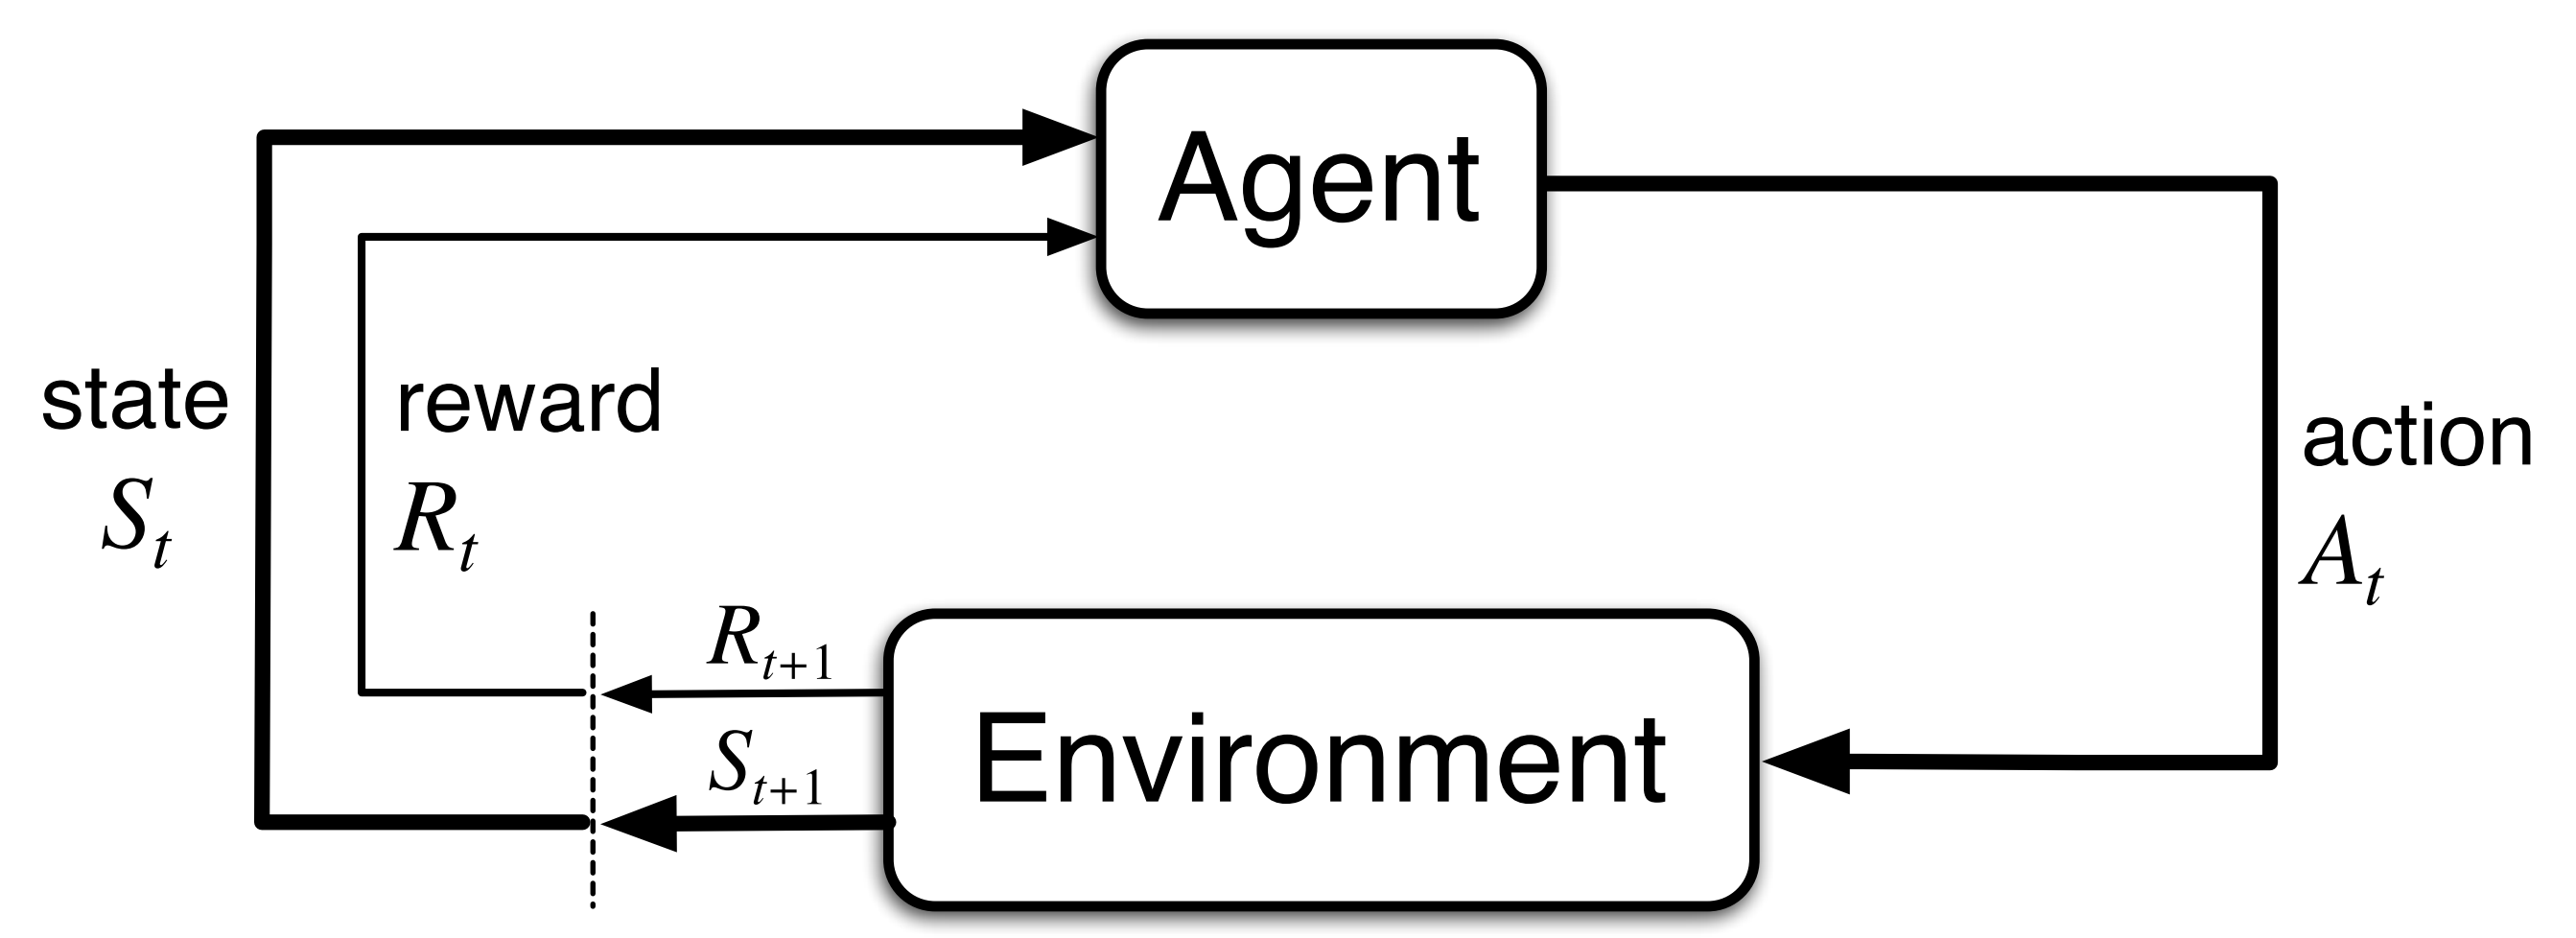
\includegraphics[width=.75\textwidth]{image/chap01/interaction.png}
		\caption{强化学习中智能体与环境的交互过程}
	\end{figure}

}

\frame{
	\begin{block}{选题的背景}
		\begin{itemize}
			\item 两类代表性经典强化学习策略更新方式:
				\begin{itemize}
					\item 以Q学习为代表的基于值函数的方式
					\item 以策略梯度为代表的基于策略的方式
				\end{itemize}
			\item 强化学习与深度学习技术的结合的成功
			      \begin{itemize}
				      \item DQN算法在Atari游戏达到了人类控制水平
				      \item AlphaGo 在围棋上战胜了人类专业棋手
			      \end{itemize}
			\item 手工设计的策略更新算法并不一定适应实际问题
		\end{itemize}
	\end{block}

	\begin{block}{选题的意义}
		\begin{itemize}
			\item[\dag] 探索新的策略更新算法,丰富强化学习的概念
		\end{itemize}
	\end{block}
	% \}
}

\subsection*{相关工作}

\frame{
	\frametitle{主流方法中的代表性工作}

	\begin{block}{MAML}
		针对小样本元学习,利用先验的优化求解过程寻找合适的初始化参数
	\end{block}

	\begin{block}{EPG}
		提出将奖励函数本身作为强化学习算法的表示的元学习框架
	\end{block}
	
	\begin{block}{LPG}
		完全舍弃基本的RL概念,利用LSTM学习一套策略更新算法
	\end{block}
}

\subsection*{本文的工作}
\frame{
	\vspace{-0.6em}
	% \begin{figure}[h]
	% 	\centering
	% 	\includegraphics[width=\textwidth]{image/illustration/networkstructure.pdf}
	% 	\caption{网络整体结构图}
	% \end{figure}
	\vspace{-1.2em}
	\begin{block}{目标与思路}
		\footnotesize
		\begin{itemize}
			\item 利用数据驱动的方式调整经典的RL算法
			\item 利用LSTM网络表示新的策略更新算法
		\end{itemize}
	\end{block}
}

